%%%%%%%%%%%%%%%%%%%%%%%%%%%%%%%%%%%%%%%%%
% Jacobs Landscape Poster
% LaTeX Template
% Version 1.1 (14/06/14)
%%%%%%%%%%%%%%%%%%%%%%%%%%%%%%%%%%%%%%%%%

\documentclass[final]{beamer}
\usepackage[ruled,vlined]{algorithm2e}
\usepackage{pstricks,pst-plot,pst-text,pst-tree,pst-eps,pst-fill,pst-node,pst-math}
\usepackage[scale=1.24]{beamerposter} % Use the beamerposter package for laying out the poster
\usetheme{confposter} % Use the confposter theme supplied with this template
\setbeamercolor{block title}{fg=ngreen,bg=white} % Colors of the block titles
\setbeamercolor{block body}{fg=black,bg=white} % Colors of the body of blocks
\setbeamercolor{block alerted title}{fg=white,bg=dblue!70} % Colors of the highlighted block titles
\setbeamercolor{block alerted body}{fg=black,bg=dblue!10} % Colors of the body of highlighted blocks

\newlength{\sepwid}
\newlength{\onecolwid}
\newlength{\twocolwid}
\newlength{\threecolwid}
\setlength{\paperwidth}{48in} % A0 width: 46.8in
\setlength{\paperheight}{36in} % A0 height: 33.1in
\setlength{\sepwid}{0.024\paperwidth} % Separation width (white space) between columns
\setlength{\onecolwid}{0.22\paperwidth} % Width of one column
\setlength{\twocolwid}{0.464\paperwidth} % Width of two columns
\setlength{\threecolwid}{0.708\paperwidth} % Width of three columns
\setlength{\topmargin}{-0.5in} % Reduce the top margin size

\usepackage{graphicx}  % Required for including images
\usepackage{booktabs} % Top and bottom rules for tables
\usepackage{pstricks,pst-plot,pst-text,pst-tree,pst-eps,pst-fill,pst-node,pst-math}

\title{Latent Dirichlet Allocation} % Poster title
\author{J\'er\^ome DOCK\`ES, Pascal LU} % Author(s)
\institute{\'Ecole Normale Sup\'erieure de Cachan $-$ \today} % Institution

\begin{document}

\addtobeamertemplate{block end}{}{\vspace*{2ex}} % White space under blocks
\addtobeamertemplate{block alerted end}{}{\vspace*{2ex}} % White space under highlighted (alert) blocks

\setlength{\belowcaptionskip}{2ex} % White space under figures
\setlength\belowdisplayshortskip{2ex} % White space under equations

\begin{frame}[t] % The whole poster is enclosed in one beamer frame

\begin{columns}[t] % The whole poster consists of three major columns, the second of which is split into two columns twice - the [t] option aligns each column's content to the top

\begin{column}{\sepwid}\end{column} % Empty spacer column

\begin{column}{\onecolwid} % The first column

%----------------------------------------------------------------------------------------
%	OBJECTIVES
%----------------------------------------------------------------------------------------

\begin{alertblock}{Objectives}
We consider the problem of modeling text corpora. The goal is to find short descriptions of the members of a collection that enable efficient processing of large collections while preserving the essential statistical relationships that are useful for basic tasks such as classification, novelty detection, summarization, and similarity and relevance judgments  \cite{BNJ03}.
\end{alertblock}

%----------------------------------------------------------------------------------------
%	INTRODUCTION
%----------------------------------------------------------------------------------------

\begin{block}{Presentation of the model}

\begin{itemize}
  \item $\mathcal{D} = \{d_{1},d_{2}, \ldots, d_{M}\}$ is a corpus.
  \item $\mathcal{V}$ is the vocabulary of size $V$.
  \item $k$ is the number of topics.
\end{itemize}

For a document $d \in \mathcal{D}$,
\begin{itemize}  
  \item $d = (w_1^{(d)}, \ldots, w_{N_d}^{(d)})$ represents the document $d$, where the $w_i^{(d)}$ are all distinct. $N_d$ is the number of \textbf{distinct} words in the document $d$.
  \item $w^{(d)}$ (\texttt{word$\_$incidences}) is a matrix containing the number of times each word in the vocabulary appears in the document. Size of $w^{(d)}$ = $N_d \times V$.
 \item $\theta^{(d)}$ is an array of size $k$, representing a probability density.
 \item $z^{(d)}$ is the set of topics : $z_{ni}^{(d)} =  1$ if the word $n$ is linked with the topic $i$. Size of $z^{(d)}$ $= N_d \times k$.
\end{itemize}

\medskip

Latent Dirichlet allocation (LDA) is a generative probabilistic model of a corpus. 
\begin{itemize}
  \item Documents = random mixtures over latent topics,
  \item Topic = a distribution over words. 
\end{itemize} 

\medskip

\begin{itemize}
  \item \textbf{Input}: {corpus $\mathcal{D}$}
\end{itemize}

For {\emph{each document} $d \in \mathcal{D}$}{

\quad Choose $N \sim \textnormal{Poisson}(\xi)$

\quad Choose $\theta^{(d)} \sim \textnormal{Dir}(\alpha)$

\quad For {\emph{each of the $N$ words $w_n^{(d)}$}}{

\quad\quad Choose a topic $z_n^{(d)} \sim  \textnormal{Multinomial}(\theta^{(d)})$

\quad\quad Choose a word $w_n$ from $p(w_n |z_n^{(d)}, \beta)$, a multi-

\quad\quad nomial probability conditioned on $z_n^{(d)}$.
}
}
\end{block}

\end{column} % End of the first column

\begin{column}{\sepwid}\end{column} % Empty spacer column

\begin{column}{\twocolwid} % Begin a column which is two columns wide (column 2)

\begin{columns}[t,totalwidth=\twocolwid] % Split up the two columns wide column

\begin{column}{\onecolwid}\vspace{-.6in} % The first column within column 2 (column 2.1)

%----------------------------------------------------------------------------------------
%	MATERIALS
%----------------------------------------------------------------------------------------

\begin{block}{Generative model}
The \textbf{goal} is to determine:

\begin{itemize}
\item $\alpha$ = estimate of the parameter of the Dirichlet distribution which generates the parameter for the (multinomial) probability distribution over topics in the document. Size of $\alpha = k$.
\item $\beta$ is a matrix of size $k \times V$ which gives the estimated probability that a given topic will generate a certain word: $\beta_{ij}= p(w^j = 1 | z^i = 1)$.
\end{itemize}

\begin{figure}[ht!]
\begin{center}
\psset{xunit=3cm,yunit=3cm,algebraic=true,dimen=middle,dotstyle=o,dotsize=5pt 0,linewidth=0.8pt,arrowsize=3pt 2,arrowinset=0.25}
\begin{pspicture*}(-0.5,-0.3)(8,3.5)
\rput(0,1){\pscirclebox[linecolor=black,fillstyle=solid,fillcolor=blue]{\textcolor{white}{$\alpha_j$}}}
\rput(2,1){\pscirclebox{$\theta^{(d)}_j$}}
\rput(4,1){\pscirclebox{$z^{(d)}_{nj}$}}
\rput(6,1){\pscirclebox[linecolor=black,fillstyle=solid,fillcolor=yellow]{$w_{nj}^{(d)}$}}
\rput(6,3){\pscirclebox[linecolor=black,fillstyle=solid,fillcolor=blue]{\textcolor{white}{$\beta_{jv}$}}}
\pspolygon(3.25,0.25)(7.2,0.25)(7.2,1.75)(3.25,1.75)
\pspolygon(1.25,0)(7.75,0)(7.75,2)(1.25,2)
\psline{->}(0.27,1)(1.58,1)
\psline{->}(2.43,1)(3.58,1)
\psline{->}(4.44,1)(5.5,1)
\psline{->}(6,2.7)(6,1.5)
\rput(6.75,0.5){$N_d$}
\rput(7.5,0.25){$M$}
\end{pspicture*}
\end{center}
\end{figure}
\end{block}

%----------------------------------------------------------------------------------------

\end{column} % End of column 2.1

\begin{column}{\onecolwid}\vspace{-.6in} % The second column within column 2 (column 2.2)

%----------------------------------------------------------------------------------------
% 
%----------------------------------------------------------------------------------------

\begin{block}{E-step for a document $d$ (Variational Inference Procedure)}

\begin{itemize}
  \item \textbf{Input}: a document $d$ defined by its \texttt{word$\_$incidences} ($w^{(d)}$), $\alpha, \beta$
  \item \textbf{Output}: $\gamma^{(d)}$, $\phi^{(d)}$
\end{itemize}

\medskip

Initialize $\phi_{ni}^{(d)} = \frac{1}{k}$ for all $i$ and $n$.

Initialize $\gamma_i^{(d)} = \alpha + \frac{1}{k}\sum_{n=1}^{N_d} w_n^{(d)}$ for all $i$.

While {\emph{the expected log-likelihood for the document $d$ has not converged}}{

\quad For {$n=1\ldots N_d$}{

\quad\quad For {$i=1\ldots k$}{

\quad\quad\quad $\phi_{ni}^{(d)} = \beta_{iw_n^{(d)}}\exp(\Psi(\gamma_i^{(d)}))$

}

\quad Normalize $\phi_n^{(d)}$ to sum to $1$.
}

\quad $\gamma^{(d)} = \alpha + \sum_{n=1}^{N_d} w_n^{(d)} \phi_n^{(d)}$
}

\end{block}

%----------------------------------------------------------------------------------------

\end{column} % End of column 2.2

\end{columns} % End of the split of column 2 - any content after this will now take up 2 columns width

%----------------------------------------------------------------------------------------
%	IMPORTANT RESULT
%----------------------------------------------------------------------------------------

%\begin{alertblock}{Important Result}

%Lorem ipsum dolor \textbf{sit amet}, consectetur adipiscing elit. Sed commodo molestie porta. Sed ultrices scelerisque sapien ac commodo. Donec ut volutpat elit.

%\end{alertblock} 

%----------------------------------------------------------------------------------------

\begin{columns}[t,totalwidth=\twocolwid] % Split up the two columns wide column again

\begin{column}{\onecolwid} % The first column within column 2 (column 2.1)

%----------------------------------------------------------------------------------------
%	MATHEMATICAL SECTION
%----------------------------------------------------------------------------------------

\begin{block}{Variational inference}

$\Rightarrow$ Use Jensen's inequality to obtain a lower bound on the log likelihood.

For a document $d \in \mathcal{D}$:
 \begin{itemize}
  \item $\gamma^{(d)}$ is the variational parameter for the dirichlet distribution. Size of $\gamma^{(d)}$ = $k$.
  \item $\phi^{(d)}$ is the variational parameter for the multinomial distribution. Size of $\phi^{(d)}$ = $N_d \times k$.
  
  $\phi_{ni}^{(d)}$ depends on the relation between the word in position $n$ of the document and the topic $i$ of the list of topics.
   \end{itemize}

$\Rightarrow$ Estimate $\gamma^{(d)}, \phi_{n}^{(d)}$ instead of $\theta^{(d)}$ and $z_n^{(d)}$.

\begin{figure}
\begin{center}
\psset{xunit=3cm,yunit=3cm,algebraic=true,dimen=middle,dotstyle=o,dotsize=5pt 0,linewidth=0.8pt,arrowsize=3pt 2,arrowinset=0.25}
\begin{pspicture*}(-1,-0.1)(4,5)
\rput(0,3){\pscirclebox[linecolor=black,fillstyle=solid,fillcolor=green]{$\gamma^{(d)}_j$}}
\rput(0,1){\pscirclebox{$\theta^{(d)}_j$}}
\rput(2,3){\pscirclebox[linecolor=black,fillstyle=solid,fillcolor=green]{$\phi^{(d)}_{nj}$}}
\rput(2,1){\pscirclebox{$z^{(d)}_{nj}$}}
\pspolygon(1.25,0.25)(3.15,0.25)(3.15,3.75)(1.25,3.75)
\pspolygon(-0.9,0)(3.8,0)(3.8,4)(-0.9,4)
\psline{->}(0,2.5)(0,1.5)
\psline{->}(2,2.5)(2,1.5)
\rput(2.75,0.5){$N_d$}
\rput(3.5,0.25){$M$}
\end{pspicture*}
\end{center}
\end{figure}

\end{block}

%----------------------------------------------------------------------------------------

\end{column} % End of column 2.1

\begin{column}{\onecolwid} % The second column within column 2 (column 2.2)

%----------------------------------------------------------------------------------------
%	RESULTS
%----------------------------------------------------------------------------------------

\begin{block}{EM-algorithm}

\begin{itemize}
  \item \textbf{Input}: {Corpus $\mathcal{D}$, number of topics $k$}
  \item \textbf{Output}: $\alpha$, $\beta$
\end{itemize}

\medskip

For each $d \in \mathcal{D}$, compute $w^{(d)}$ (\texttt{word$\_$incidences}).

Initialize $\alpha$, $\beta$ and $\Sigma_{\gamma}$ = 0.

\medskip

While {\emph{the expected log-likelihood has not converged}: }{

\quad For {\emph{each} $d \in \mathcal{D}$}{

\quad\quad ($\gamma^{(d)}$, $\phi^{(d)}$) = \textbf{E-step}($w^{(d)}$, $\alpha$, $\beta$)

\quad\quad Update $\beta \leftarrow \beta +  (\phi^{(d)})^{\top}w^{(d)}$

\quad\quad Update $\Sigma_{\gamma} \leftarrow \Sigma_{\gamma} + \sum_{i=1}^k \Psi (\gamma_i^{(d)}) - \Psi\left( \sum_{j=1}^k \gamma_j^{(d)}\right) $
}

\quad Normalize $\beta$ 

\quad While {\emph{$\alpha$ has not converged}}{

\quad \quad $\alpha \leftarrow \alpha - \frac{L'(\alpha)}{L''(\alpha)}$ where \[ \begin{cases}L'(\alpha) = |\mathcal{D}| k \left[ \Psi\left( k \alpha \right) - \Psi(\alpha)\right] + \Sigma_{\gamma} \\
L''(\alpha) = |\mathcal{D}|k [k\Psi'(\alpha) - \Psi' \left( \alpha\right)] \end{cases} \]

}
}
\end{block}

\begin{block}{Implementation issues}
\begin{itemize}
  \item Initialization of $\alpha$ et $\beta$.
  \item Optimization and convergence of the parameters and the expected log-likelihood.
\end{itemize}
\end{block}

%----------------------------------------------------------------------------------------

\end{column} % End of column 2.2

\end{columns} % End of the split of column 2

\end{column} % End of the second column

\begin{column}{\sepwid}\end{column} % Empty spacer column

\begin{column}{\onecolwid} % The third column

%----------------------------------------------------------------------------------------
% RESULTS
%----------------------------------------------------------------------------------------

\begin{block}{Results}

We have tested our algorithm on real data from the Reuters21578 database.

\begin{table}
\vspace{2ex}
\begin{small}
\begin{tabular}{c c c c}
\toprule
\textbf{Topic 1} & \textbf{Topic 2} & \textbf{Topic 3}  & \textbf{Topic 4}\\
\midrule
devices & prolonged & zestril & features \\
disk & council & annesthetic &  shipping  \\
megabyte & forum & hypertension & 798  \\
expandable & dissident & oth & 998  \\
megabytes & flying & statil & sells  \\
equipped &  sparks & diabetic & AppleWorld  \\
monochrome &talks & complications & Conference  \\
peripheral & outweighed & Barbara & 899  \\
color & accomplishments & definitive & science  \\
\bottomrule
\end{tabular}
\end{small}
\caption{Results for 4 topics}
\end{table}

\begin{figure}[ht!]
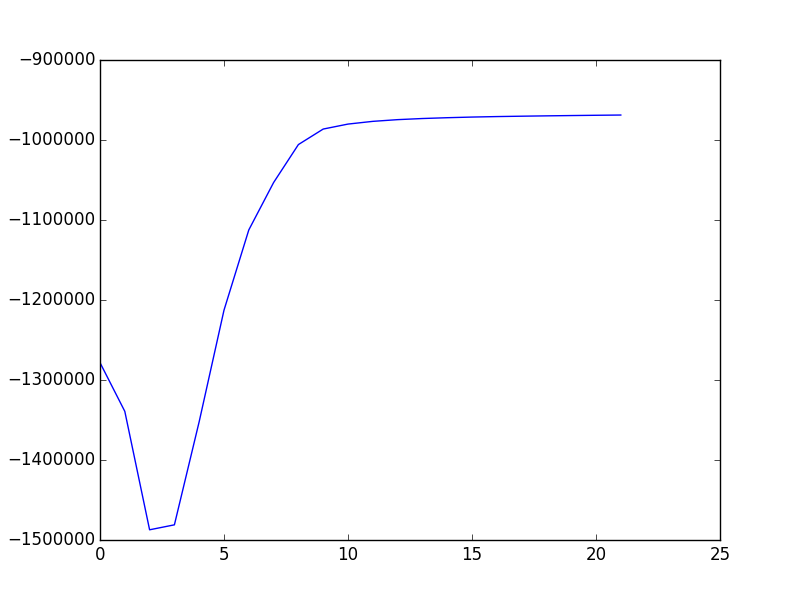
\includegraphics[width=0.5\linewidth]{../img/figure_1.png}
\caption{Expected log-likelihood for a corpus, $k=30$}
\end{figure}

\begin{figure}[ht!]
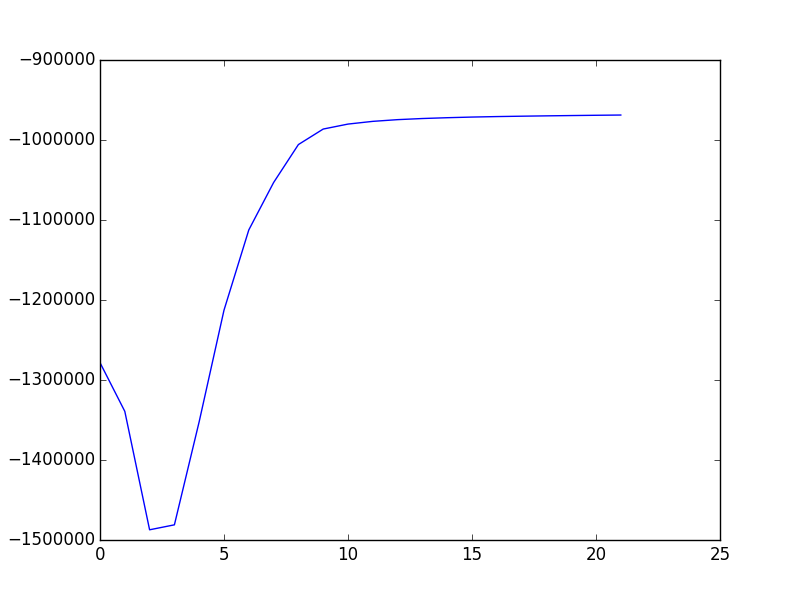
\includegraphics[width=0.5\linewidth]{../img/figure_1.png}
\caption{Expected log-likelihood for a document, $k=30$}
\end{figure}

\end{block}

%----------------------------------------------------------------------------------------
%	CONCLUSION
%----------------------------------------------------------------------------------------

\begin{block}{Conclusion}

\end{block}

%----------------------------------------------------------------------------------------
% REFERENCES
%----------------------------------------------------------------------------------------

\begin{block}{References}

\nocite{*} % Insert publications even if they are not cited in the poster
\small{\bibliographystyle{unsrt}
\bibliography{sample}\vspace{0.75in}}

\end{block}

%----------------------------------------------------------------------------------------
% CONTACT INFORMATION
%----------------------------------------------------------------------------------------

\setbeamercolor{block alerted title}{fg=black,bg=norange} % Change the alert block title colors
\setbeamercolor{block alerted body}{fg=black,bg=white} % Change the alert block body colors

%\begin{alertblock}{Contact Information}
%\begin{itemize}
%  \item \texttt{jerome\{at\}dockes.org}
%  \item \texttt{pascal.lu\{at\}centraliens.net}
%\end{itemize}
%\end{alertblock}

%----------------------------------------------------------------------------------------

\end{column} % End of the third column

\end{columns} % End of all the columns in the poster

\end{frame} % End of the enclosing frame

\end{document}
